% +---------------------------------------------------------------+
% | Author :    Noémie Plancherel, HEIG-VD
% | Date :      20.09.2022
% +---------------------------------------------------------------+

\chapter{Sélection des candidats}
\label{ch:selection}
Dans ce chapitre, nous allons faire la sélection des gestionnaires de mots de passe que nous analyserons dans le
chapitre suivant. Nous définirons les critères des sélections afin de correctement les choisir, puis nous ferons
notre choix en fonction des candidats sélectionnés. Afin d'avoir une bonne vue d'ensemble sur les fonctionnalités et
la sécurité de chaque application, nous allons reprendre les 9 gestionnaires analysés dans les chapitres précédents.

\section{Critères de sélection}

Cette section va ainsi présenter les critères de sélections pour les candidats avec lesquels on fera une analyse
sécuritaire détaillée.

\textbf{Open-source} - un critère assez important car un gestionnaire de mots de passe open-source pourrait être plus
sûr qu'un gestionnaire closed-source dû au fait qu'importe quel utilisateur peut auditer le code source
indépendamment et peut reporter des failles aux constructeurs. Les applications closed-source comptent à 100\% sur
l'équipe de développement et pourrait faire face à plus d'attaques.

\textbf{Types} - nous allons sélectionner des gestionnaires des 3 types différents afin d'avoir un éventail complet
de gestionnaires de mots de passe existants. Pour faire un rappel, les différents types sont: cloud-based,
local-based et browser-based.

\textbf{Gratuit} - il est bien de prendre en compte ce critère afin d'analyser si un gestionnaire proposant des
fonctionnalités gratuites est plus faible qu'un gestionnaire complètement payant. De plus, il pourrait être
intéressant de comparer la sécurité d'un application qui propose des fonctionnalités gratuites et payantes.

\textbf{Nombre d'utilisateurs} - il est intéressant d'ajouter le critère de la popularité afin de se rendre compte
de l'impact de quelconques vulnérabilités présentes sur l'application et de constater malgré une grande
popularité, s'il y a l'existence de failles non-corrigées ou non-prises en compte.

\textbf{Partage de données} - cette fonctionnalité est assez critique, dû au fait que des données sont partagées
entre plusieurs utilisateurs, il est impératif que les données soient uniquement accessibles par les bonnes personnes
de confiance. Ainsi, il serait intéressant de sélectionner au moins un candidat qui propose cette fonctionnalité pour
évaluer la sécurité.

\textbf{Choix cryptographiques} - ce critère concerne les choix cryptographiques utilisés pour le chiffrement des
données par exemple, ou la dérivation des clés. Il sera important d'évaluer si ces choix sont suffisant. Ainsi, nous
allons sélectionner des candidats qui ont effectuer des choix cryptographiques différents.

\textbf{Plateforme supportée} - l'analyse sécuritaire se fera dans un premier temps sur un ordinateur avec Windows
11, donc les applications doivent être disponibles pour cet OS. La raison pour laquelle nous faisons ce choix est que c'est un des OS les plus populaires sur le marché.

\textbf{Failles connues} - pour quelques gestionnaires de mots de passe, des vulnérabilités ont été découvertes. Pour
certaines, des corrections ont été faites aux applications mais certaines n'ont pas été corrigée malgré un report
vers les constructeurs des gestionnaires. Ainsi, ceci est un aspect important à prendre en compte afin de constater
si les failles ont été corrigées après leurs découvertes.

\section{Choix}
Afin d'avoir une bonne vue d'ensemble sur tous les candidats et de faire une sélection pertinente, nous allons
établir un tableau récapitulatif. Lors du choix, nous allons tenter de couvrir tous les critères proposés avant, afin
de faire une analyse complète et diverse sur tout ce qui existe sur le marché actuellement.

Nous allons donc choisir X candidats pour avoir une bonne vue d'ensemble sur tout ce qui existe.

\begin{figure}[H]
	\centering
	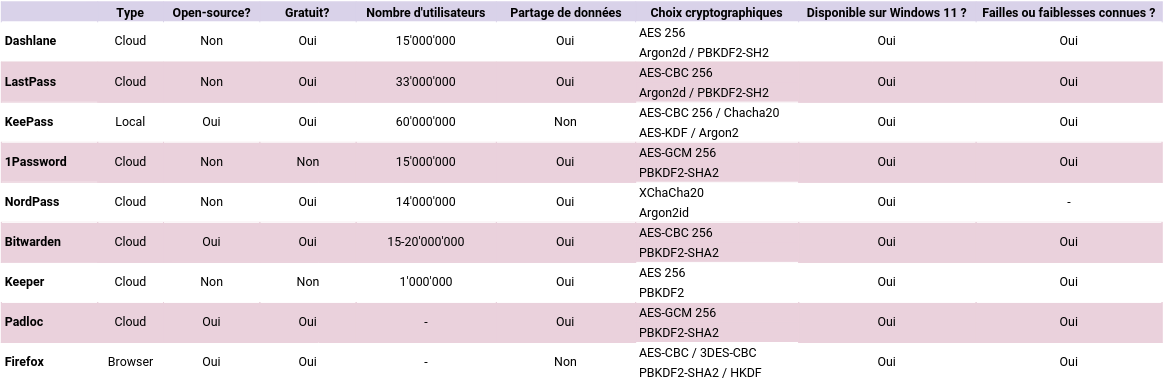
\includegraphics[scale=0.5, angle=90]{images/selection_choix.png}
	\caption{Comparatif des candidats pour la sélection}
\end{figure}

Ainsi, nous allons sélectionner:
\begin{itemize}
	\item LastPass
	\item KeePass
	\item Firefox
	\item 1Password
\end{itemize}

Chaque chapitre dédié aux gestionnaires de mots de passe sélectionnés se basera sur les exigences sécuritaires que nous avons définis au chapitre précédent et sur les vulnérabilités et faiblesses déjà connues. 

À chaque début de chapitre, nous établirons les critères d'évaluation de la sécurité de l'application. Les critères seront à chaque fois différents en fonction du type ou des fonctionnalités proposées. 


